\lecture{11}{3. Marts 2025}{Introduction to Polymer Science – By guest-lecturer Simon Mckie}

\section{Polymer Chemistry}
Polymers are long chains of covalently bonded monomers. The interactions between these polymers define the characteristics of the polymer. Two common monomers you will find in nature is cellulose (fibers in plants and grasses) and isoprene (found in the sap of rubber trees). The same monomers does not necessarily give the same properties of the polymer -- e.g. nitrocellulose and camfer makes billiard balls whereas nitrocellullose and octasulfur gives tire-rubber. 

The process of converting a bunch of monomers into polymers one must normally let the monomers be in a high-temperature high-pressure environment for the reaction to occur.

\begin{definition}[Polymer]
  A polymer is the main ingredient in \textit{plastics}. Polymers are long chains of monomers (small ``unit''-atoms). The word ``polymer'' comes from greek polús meaning ``many'' and greek méros meaning ``parts''. Plastics are made up of polymers and additives.
\end{definition}

To make ABS -- such as at LEGO. One needs to combine the monomers of \textit{acrylonitrile}, \textit{butadiene}, and \textit{styrene}. To make polyethylene you just need the monomer ``ethylene''.

\subsection{Polymerisation}
To make plastics, one needs to polymerize some monomers, as mentioned above. There is broadly two types of polymerisation, i.e. addition and condensation polymerisation. 

\subsubsection{Addition polymerisation}
On \textbf{\autoref{fig:f11_1}} two different addition polymerisations are shown. These are all characterized by an addition reaction being the main reaction type driving the polymerisation. 

\begin{figure} [ht]
  \centering
  \caption{Two different addition polymerisations}
  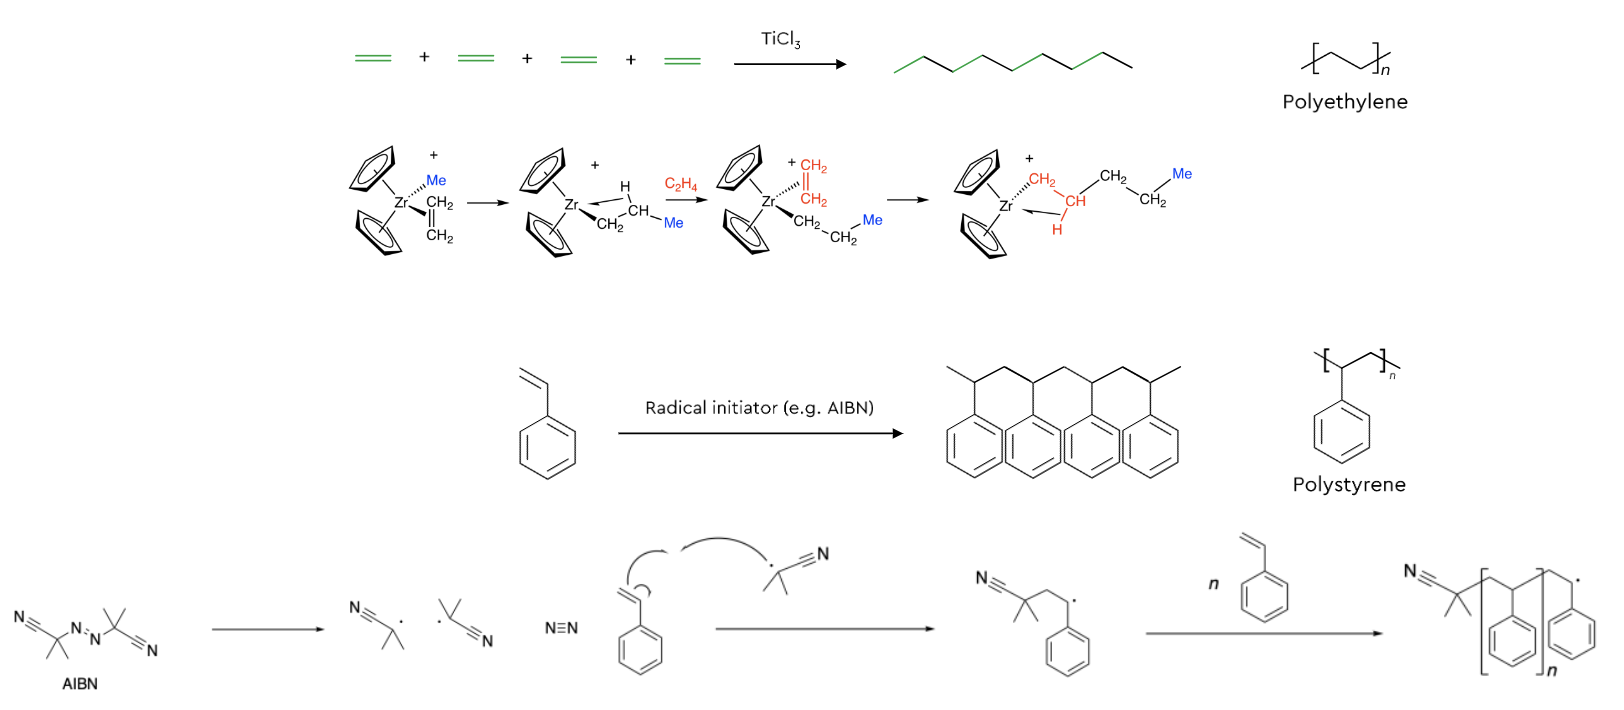
\includegraphics[width=0.75\linewidth]{./figures/f11_1.png}
  \label{fig:f11_1}
\end{figure}

\subsubsection{Condensation polymerisation}
On \textbf{\autoref{fig:f11_2}} a condensation polymerisation is shown. These are characterized by condensation reactions and therefore small amounts of additional ``product'' is made during the reaction -- this can be but is not necessarily water. 

\begin{figure} [ht]
  \centering
  \caption{A condensation polymerisation}
  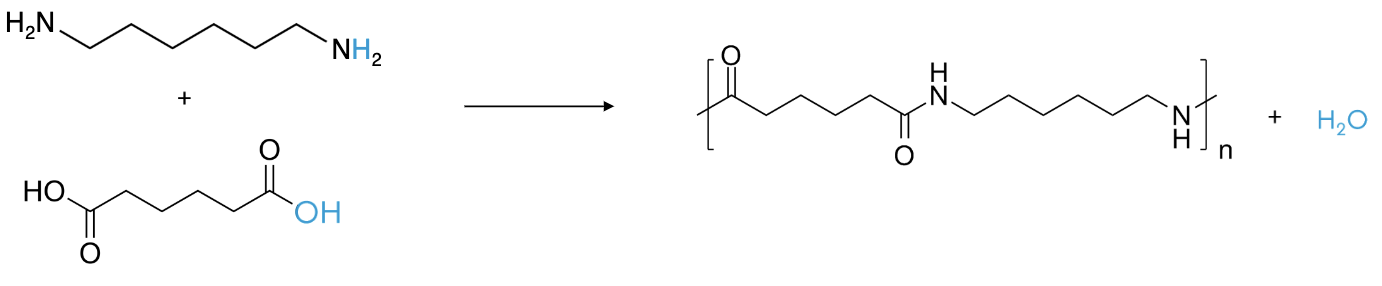
\includegraphics[width=0.5\linewidth]{./figures/f11_2.png}
  \label{fig:f11_2}
\end{figure}

\subsection{Polymer lengths and length distribution}
There are a few definitions that we need to get under our belt before continuing.
\begin{definition}[Average molecular weight]
  The average molecular weight in a polymer is the average mass of the polymer chains.
\end{definition}
\begin{definition}[Molecular weight distribution]
  The molecular weight distribution is how the molecular weights of the polymer chains are distributed.
\end{definition}
\begin{definition}[Degree of polymerisation]
  The degree of polymerisation is a measurement for the number of monmeric units in the polymer chains.
\end{definition}

\subsubsection{Molecular weight and reaction speed}
On \textbf{\autoref{fig:f11_3}} the difference in reaction speed between the step growth type polymerisation and chain-growth polymerisation.
\begin{figure} [ht]
  \centering
  \caption{Difference between step-growth and chain-growth}
  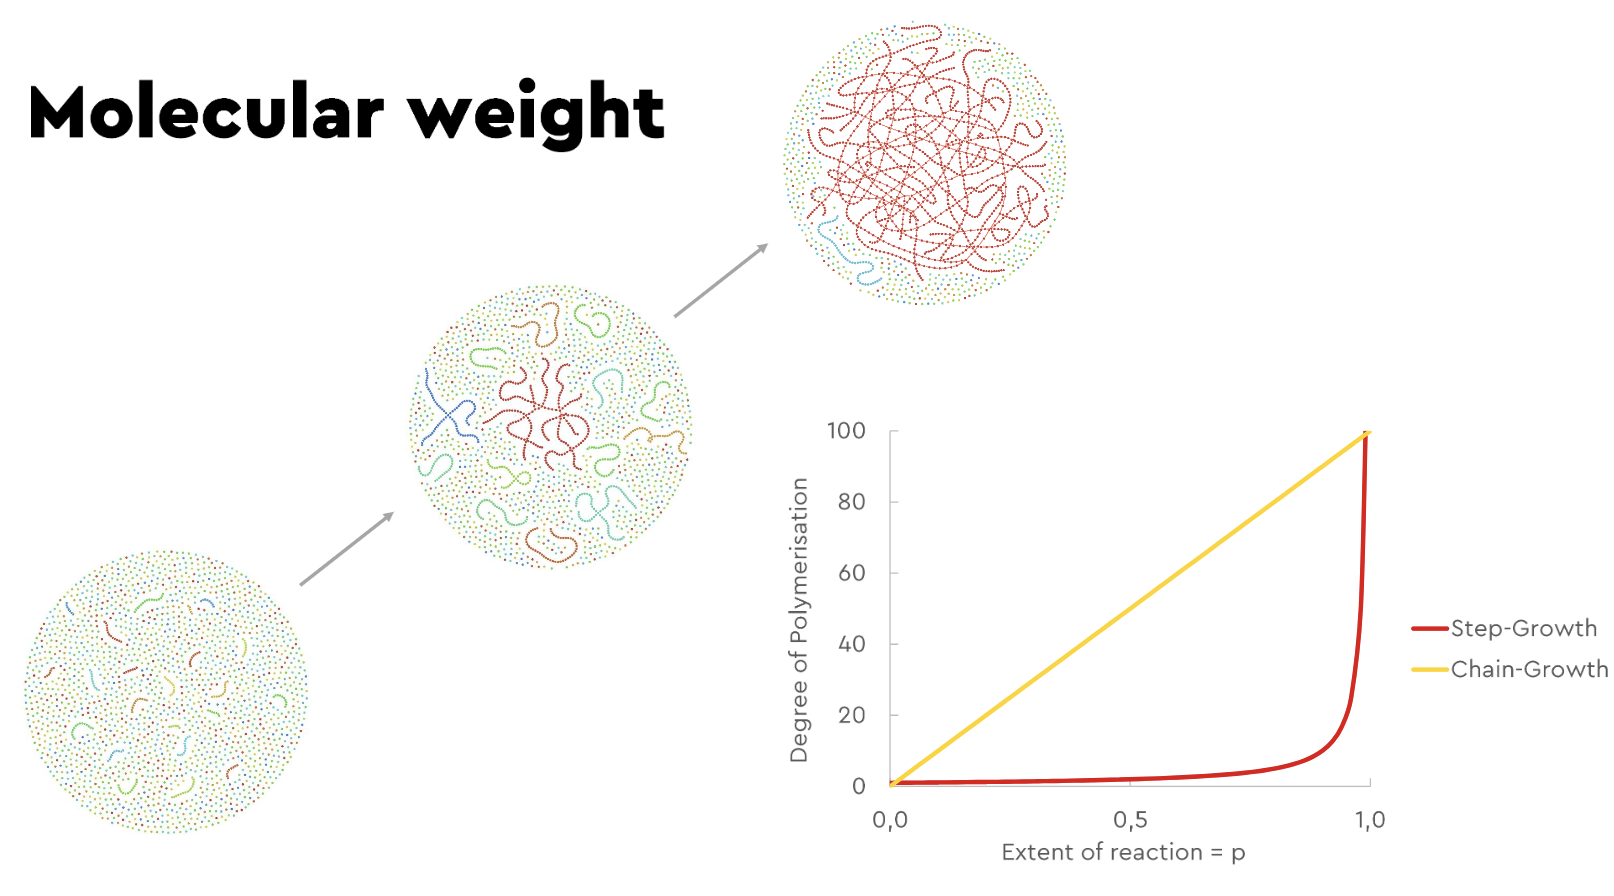
\includegraphics[width=0.75\linewidth]{./figures/f11_3.png}
  \label{fig:f11_3}
\end{figure}

\subsubsection{Molecular weight distribution}
When polymerising a bunch of monomers you cannot expect all monomers to react exactly the same. Instead one might imagine a normally-distributed mass-distribution around some average value. This is shown on \textbf{\autoref{fig:f11_4}} and \textbf{\autoref{fig:f11_5}} (the molecular weight of the monomer is around \qty{28}{g/mol} in this case). The difference between \textbf{\autoref{fig:f11_4}} and \textbf{\autoref{fig:f11_5}} is that on \textbf{\autoref{fig:f11_4}} the ``number average'' molecular weight has been found using the formula
\[ 
M_n = \sum x_i M_i
\]
whereas the ``weight average'' molecular weight on \textbf{\autoref{fig:f11_5}} has been found using
\[ 
M_w = \sum w_i M_i
.\]
These are in many ways equivalent, although the weight average will be skewed towards heavier molecules compared to the number average.
\begin{figure} [ht]
  \centering
  \caption{Number average molecular weight distribution}
  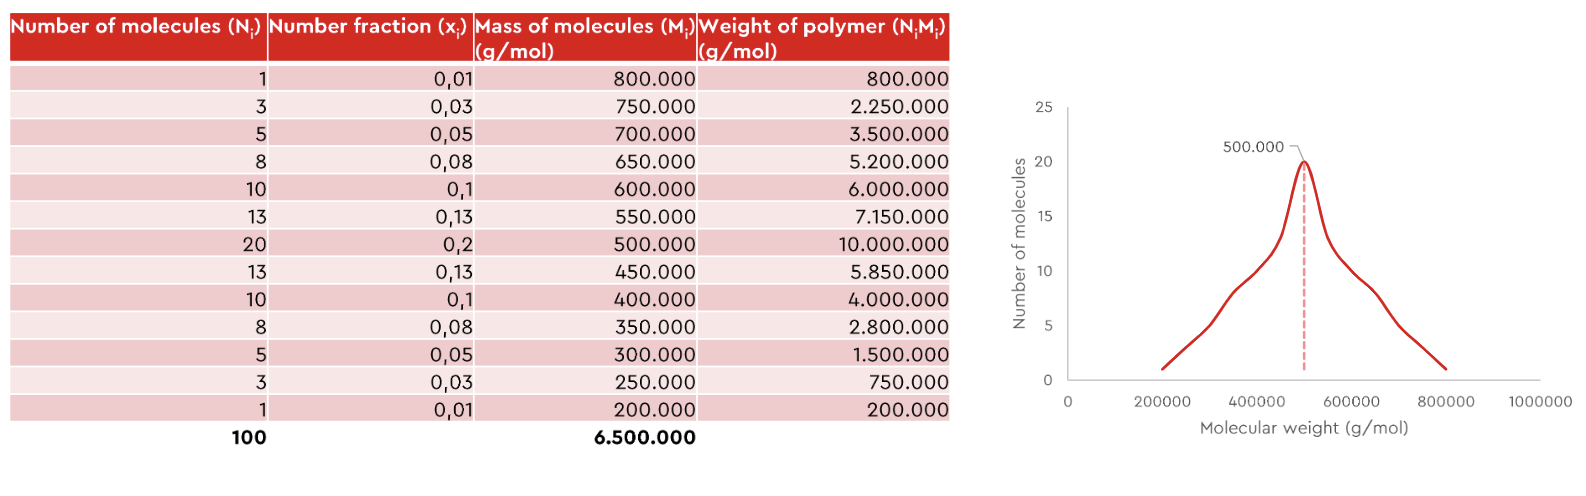
\includegraphics[width=0.75\linewidth]{./figures/f11_4.png}
  \label{fig:f11_4}
\end{figure}
\begin{figure} [ht]
  \centering
  \caption{Weight average molecular weight distribution}
  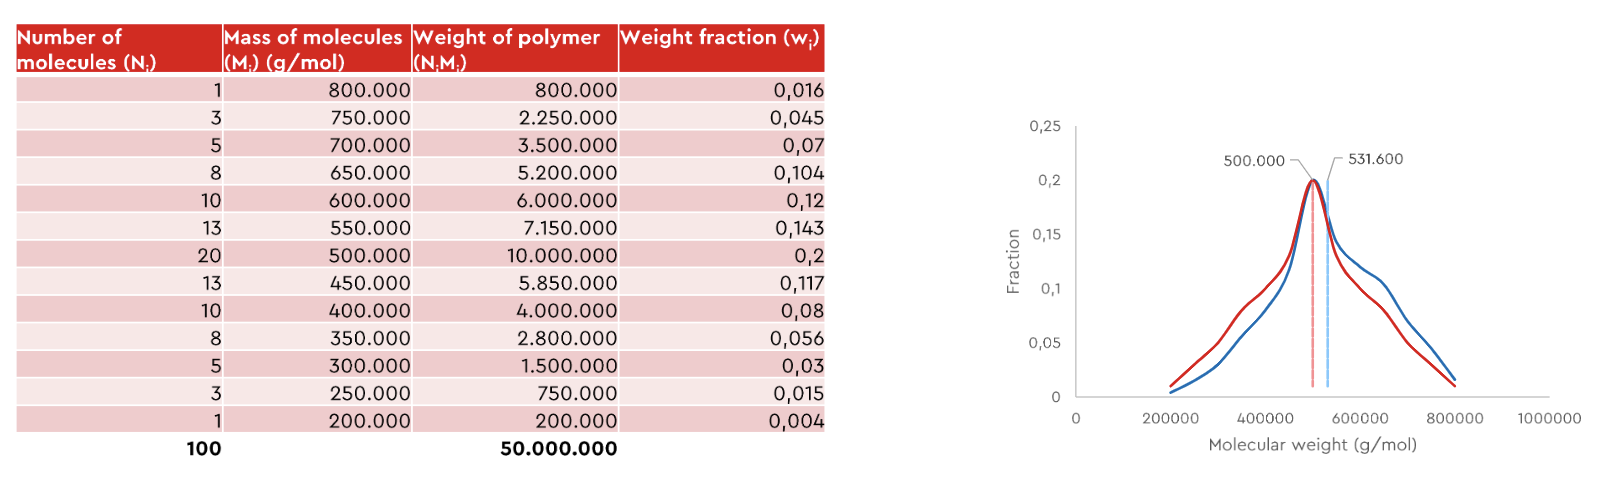
\includegraphics[width=0.75\linewidth]{./figures/f11_5.png}
  \label{fig:f11_5}
\end{figure}

The relationship between the number average molecular weight and the weight average molecular weight is given by the index of dispersity, $\mathrm{PDI}$ (disperisty factor). This is given by
\[ 
\mathrm{PDI} = \frac{M_w}{M_n}
.\]

\subsubsection{Degree of polymerisation}
The degree of polymerisation can simply be found as
\[ 
\frac{M_n}{M_0}
\]
where $M_0$ is the molecular weight of the monomer.

\subsubsection{Material properties and molecular weight}
In general the tensile strength, impact strength and viscosity are all increasing for increasing molecular weights. This is shown on \textbf{\autoref{fig:f11_6}}.
\begin{figure} [ht]
  \centering
  \caption{The influence of molecular weight on material properties}
  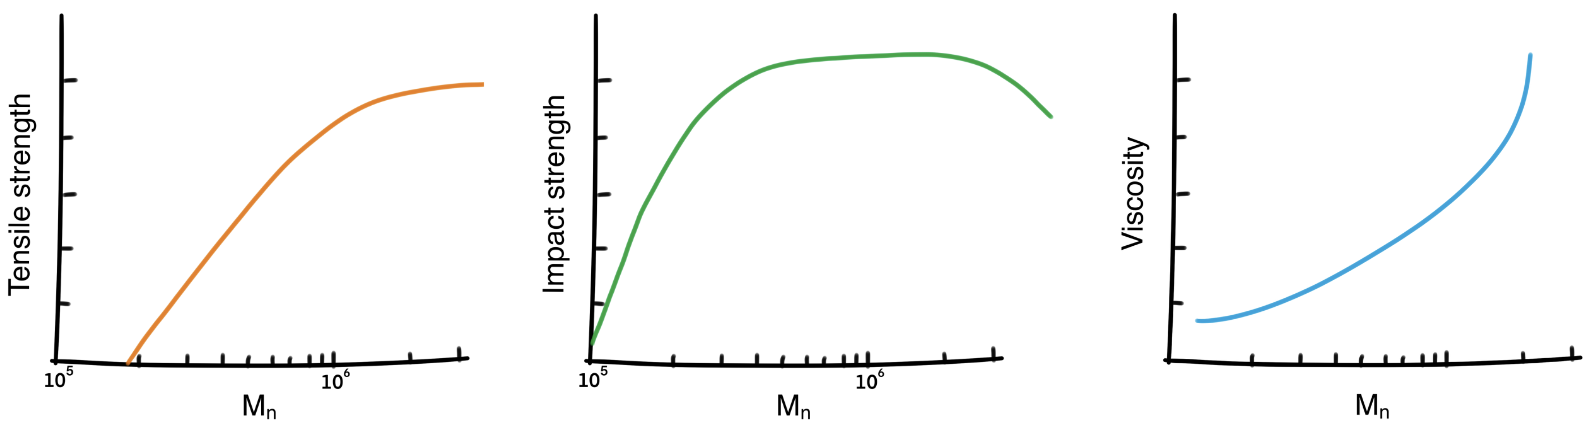
\includegraphics[width=0.75\linewidth]{./figures/f11_6.png}
  \label{fig:f11_6}
\end{figure}

\begin{exa}[Index of dispersity and molecular weights]
  We want to determine the degree of polymerisation in a sample of polyethylene with a mass-average molecular mass of \qty{196400}{g/mol}. We know that $\mathrm{PDI} \leq \num{1,2}$.
  \bigbreak
  To start we use the dispersity to calculate the number average molecular mass as
  \begin{align*}
    \mathrm{PDI} &= \frac{M_w}{M_n} \\
    M_n &= \frac{M_w}{\mathrm{PDI}} \\
    &= \frac{\qty{196400}{\frac{g}{mol}}}{\num{1,2}} \\
    &= \qty{163666,66}{\frac{g}{mol}} 
  .\end{align*}
  We can now find the degree of polymerisation as
  \begin{align*}
    \text{deg. polym.} &= \frac{M_n}{M_0} \\
    &= \frac{\qty{163666,66}{\frac{g}{mol}}}{\qty{28,06}{\frac{g}{mol}} } \\
    &= \num{5832,7} 
  .\end{align*}
\end{exa}

\subsection{Mixing polymers}
Until now we have only focused on polymers consisting of only one polymer. A \textit{blend} or a \textit{compound} is a mixture between two or more polymers. Long large macromolecules have a rather low entropy and therefore blending two polymers is thermodynamically often rather hard (as the Gibbs free energy is not negative for low entropy) -- but sometimes it can give desired effects. Blends or compounds are also often known as \textit{co-polymers}.

When mixing two polymers they can either be miscible (rare) or immiscible (common) as shown on \textbf{\autoref{fig:f11_7}}. To combat this one can add an emulsifier or an ``emulsifying polymer'' to help with the blending.
\begin{figure} [ht]
  \centering
  \caption{Miscible and immiscible polymers}
  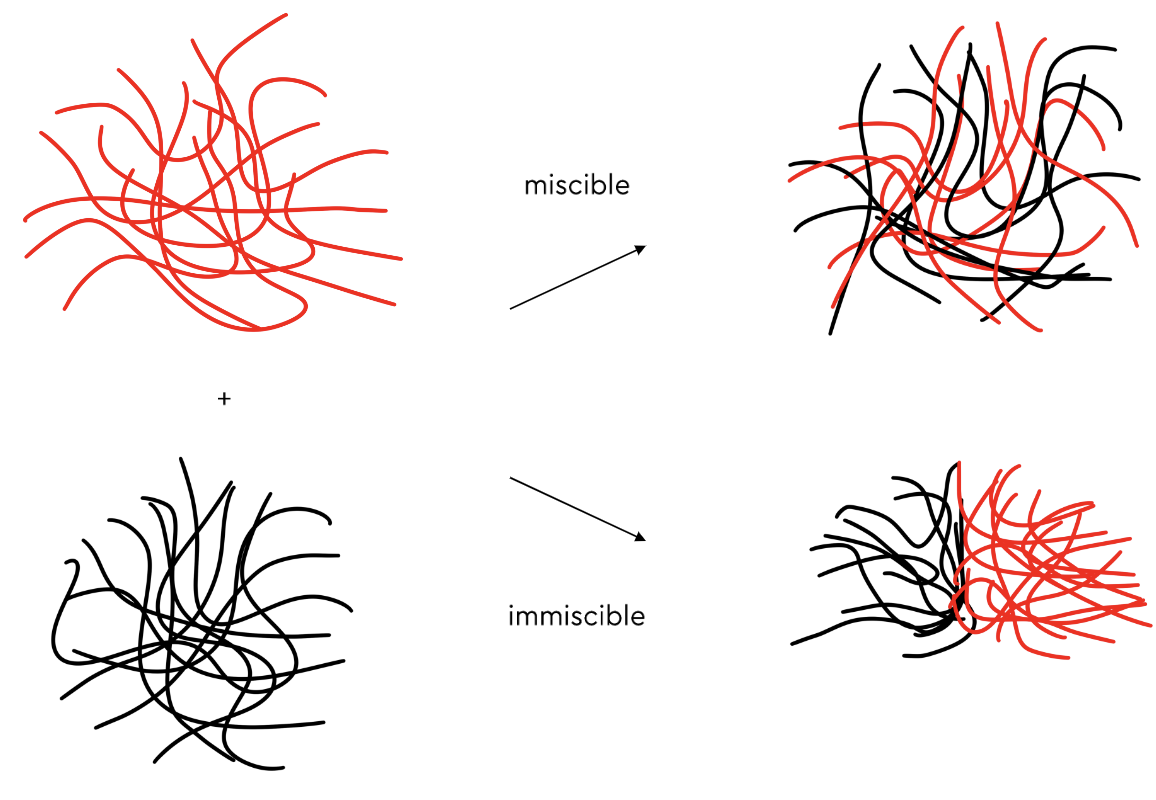
\includegraphics[width=0.5\linewidth]{./figures/f11_7.png}
  \label{fig:f11_7}
\end{figure}
An example of the ``emulsifying polymer'' described above is used when mixing polybutadiene and styrene acrylonitrile to make ABS. These are normally immiscible and therefore something must be done for the two polymers to mix and not just form a two-phase mix. What is done in practise is that one can ``graft'' styrene acrylonitrile chains to the polymer chain of polybutadiene chemically. This means that the acrylonitrile and the polybutadiene are bonded together chemically and the acrylonitrile polymers can now grow from the grafted ``nucleation points''. 

\section{Polymer Processing and Conversion}
When wanting to make a polymer you typically start with oil, which you refine into monomers and then polymerize into polymers. For condensation polymerisation one needs to keep in mind, that it is an equilibrium reaction -- therefore it is important to drive off the biproduct formed during the reaction (e.g. with a vacuum to suck away water). This however is not only a bad thing. The fact that the reaction is reversible means that one can break down the polymers in a condensation polymer by adding the biproduct back again and this way one can recycle used condensation polymers easier than addition polymers.

\begin{definition}[Glass transition temperature]
  The \textit{glass transition temperature} is the equivalent of a melting point for an amorphous material.
\end{definition}

Polymers are (often) non-newtonian meaning that their viscosity changes with the flow speed -- polymers are shear thinning, meaning that the more you shear (the faster you try to make it flow) the thinner the polymer will become. This is shown on \textbf{\autoref{fig:f11_8}}. This happens because the high temperature decreases the influence of e.g. Van der Waals-interactions between the polymer chains.
\begin{figure} [ht]
  \centering
  \caption{Shear thinning of polymers}
  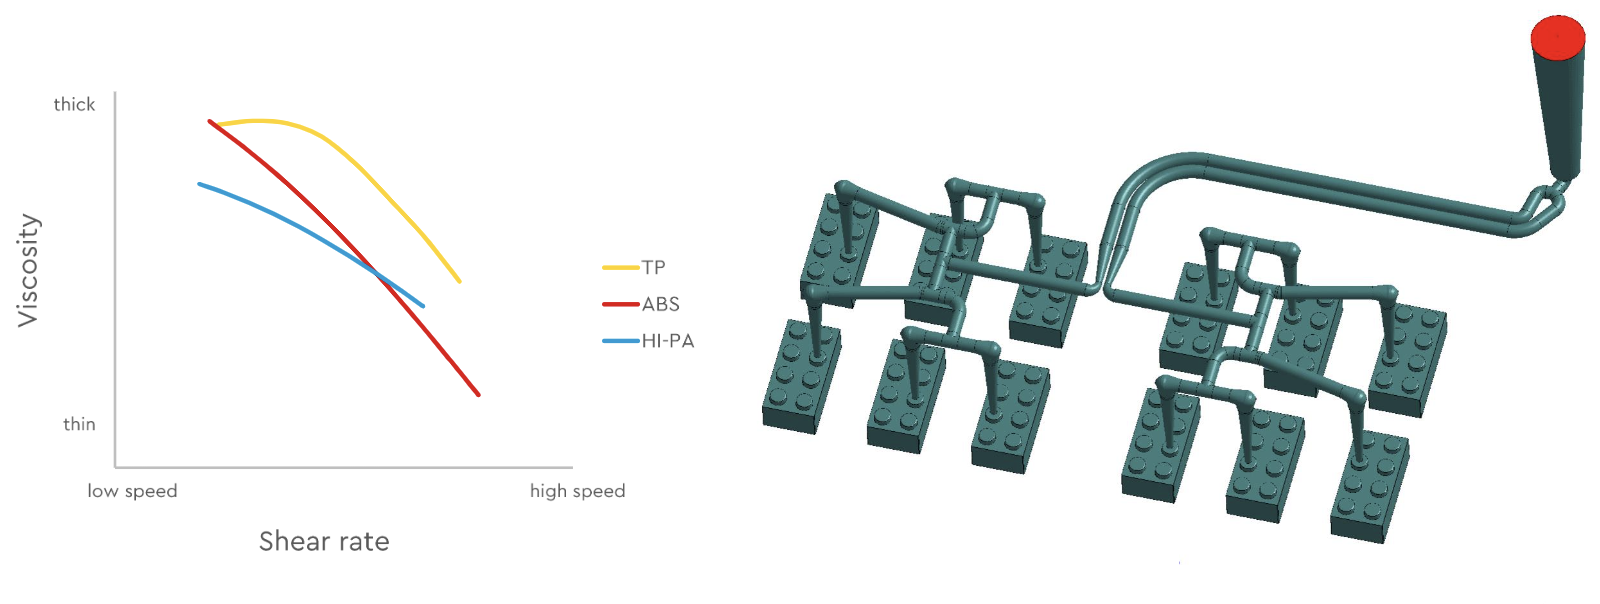
\includegraphics[width=0.75\linewidth]{./figures/f11_8.png}
  \label{fig:f11_8}
\end{figure}
